\documentclass[10pt]{article}

\title{ITF31519 - Assignment 2}
\author{Tobias Hallingstad}

\usepackage[utf8]{inputenc}
\usepackage[english]{babel}
\usepackage{minted}

\usepackage{graphicx}
\graphicspath{ {./images/} }

\begin{document}
    \begin{titlepage}
        \maketitle
    \end{titlepage}

    \newminted{python}{
        gobble=2,
        linenos
    }

    \section{Default values}
    I am basing the \texttt{MLPClassifier} on some default values. Thease values are used if no other value is sepefied: \texttt{randomState = 1, maxIter = 300, nLayers = (100,)}

    \section{Observations}
        \paragraph{Number of nodes}
        I did some testing on what effect the amount of nodes have on the model. I wrote a function (\texttt{plotMulti2()}) to run multiple itterations of the model (with different number of nodes), then plot the resoult in a bar diagram. Here I run 15 diffrent models, where i increase the ammount of nodes in the first layer.

        \begin{center}
            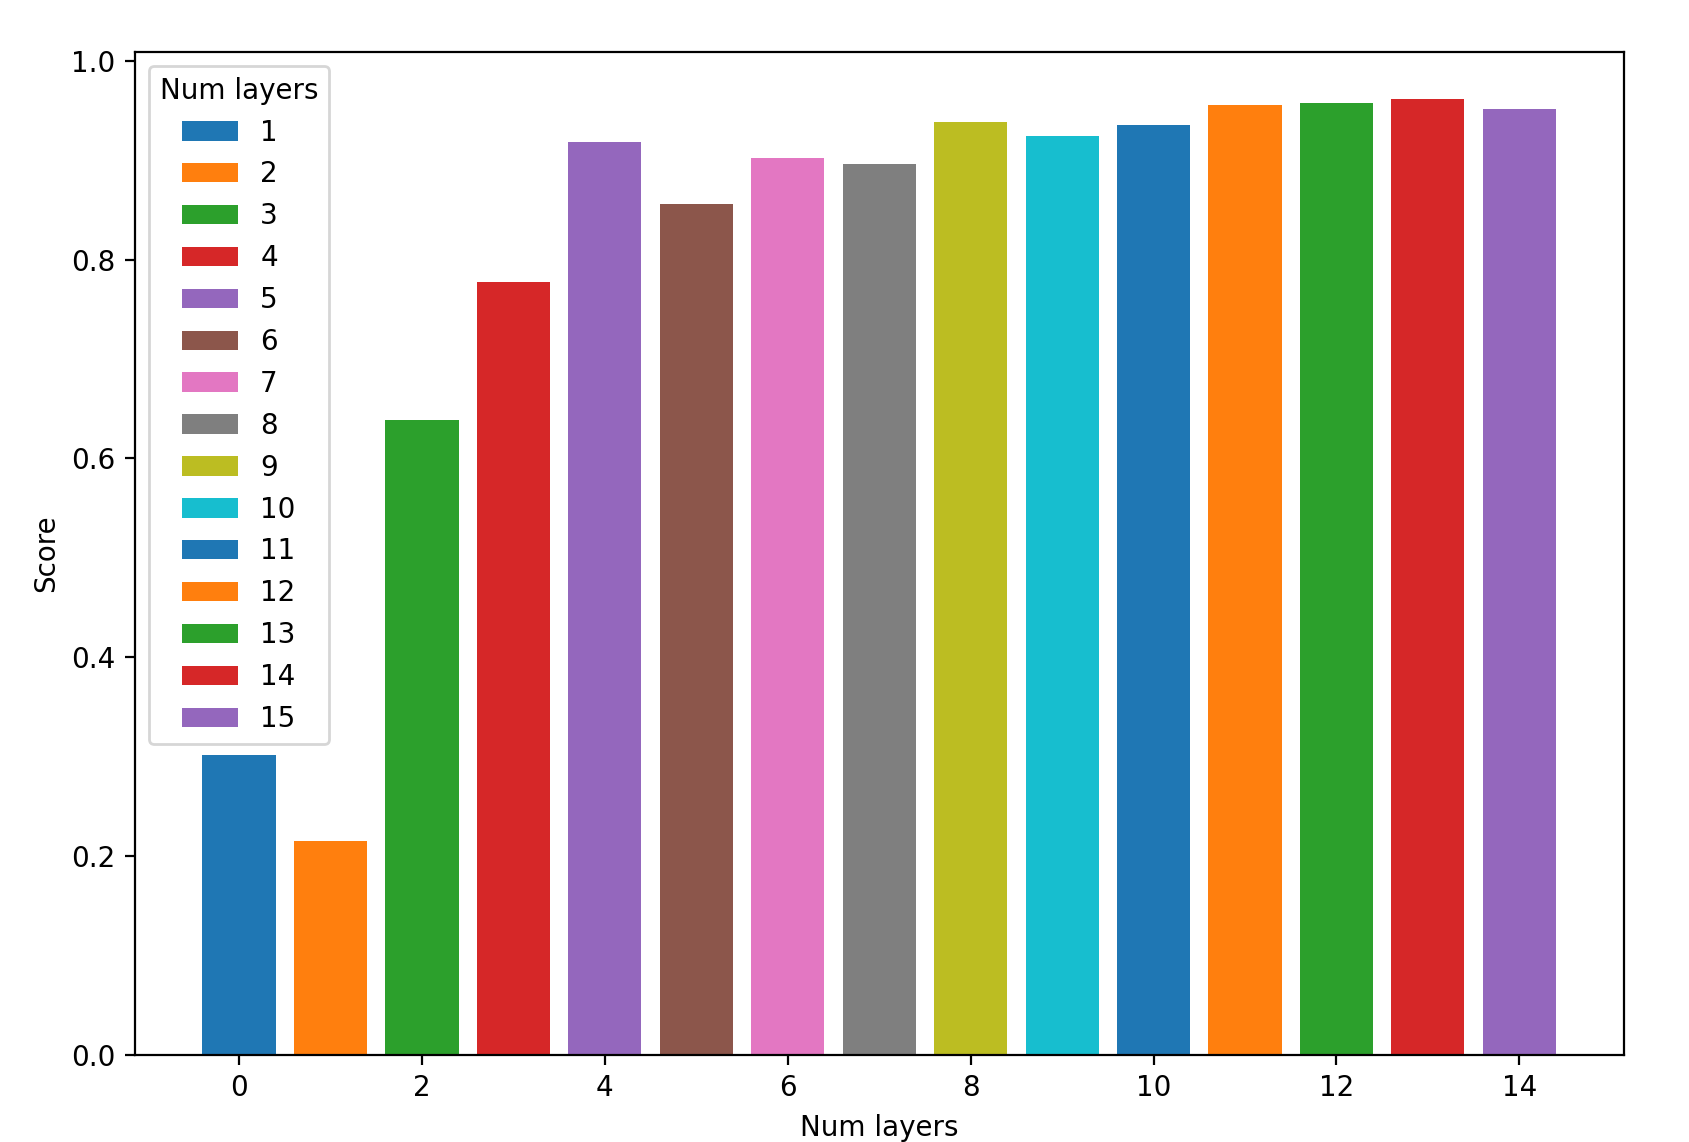
\includegraphics[scale=0.35]{Figure_1}
        \end{center}

        Here I can see that afther 8 nodes there is litle change in the score.

        \paragraph{Numer of hidden layers}
        Afther testing how many nodes in 1 layer looks good. I proseeded to test how many hidden layers I can use with 8 nodes in. For this I uesd the \texttt{plotMulti3()}. Here I played around with the \texttt{iterations} variable to finde some interesting data. I here use 150 to se if that changes the score.

        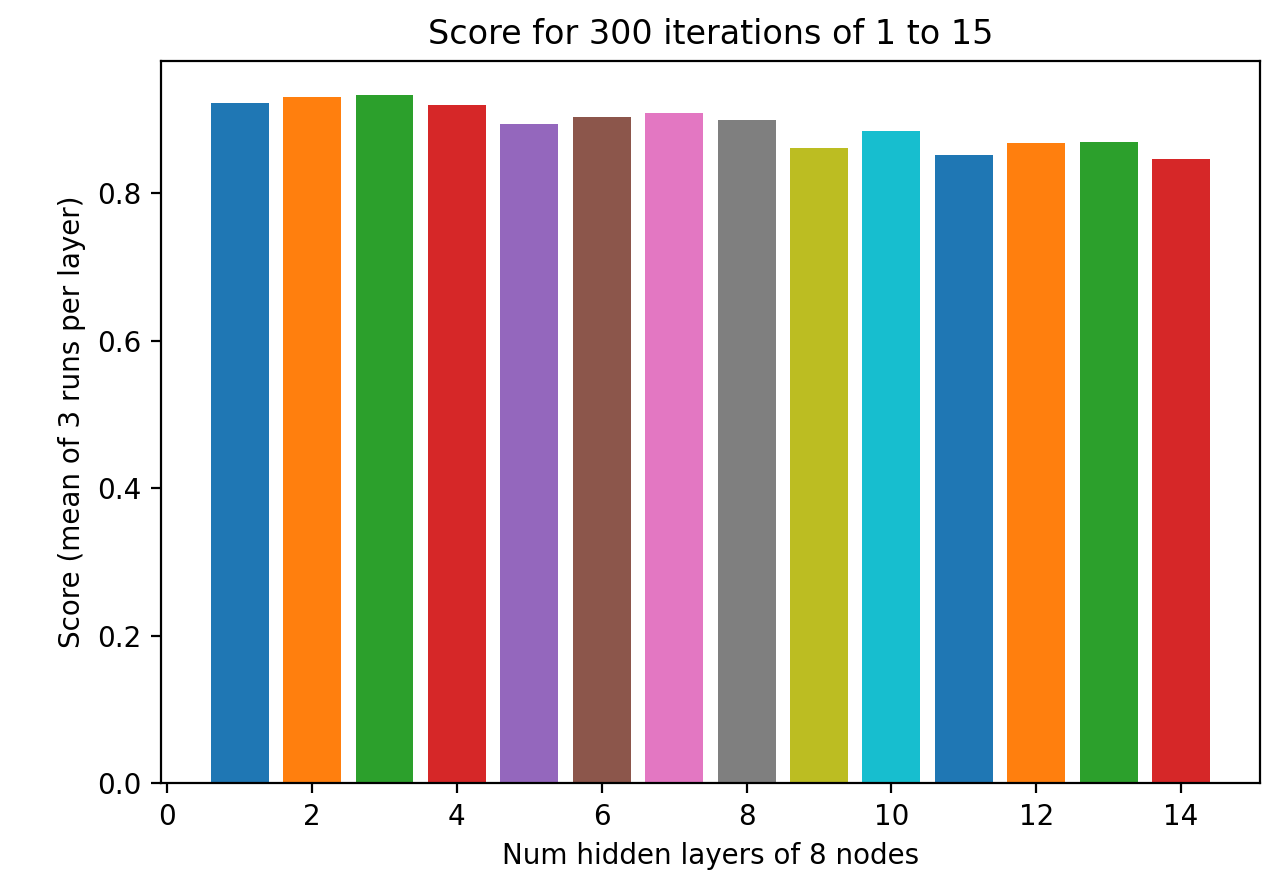
\includegraphics[scale=0.4]{Figure_2-1}
        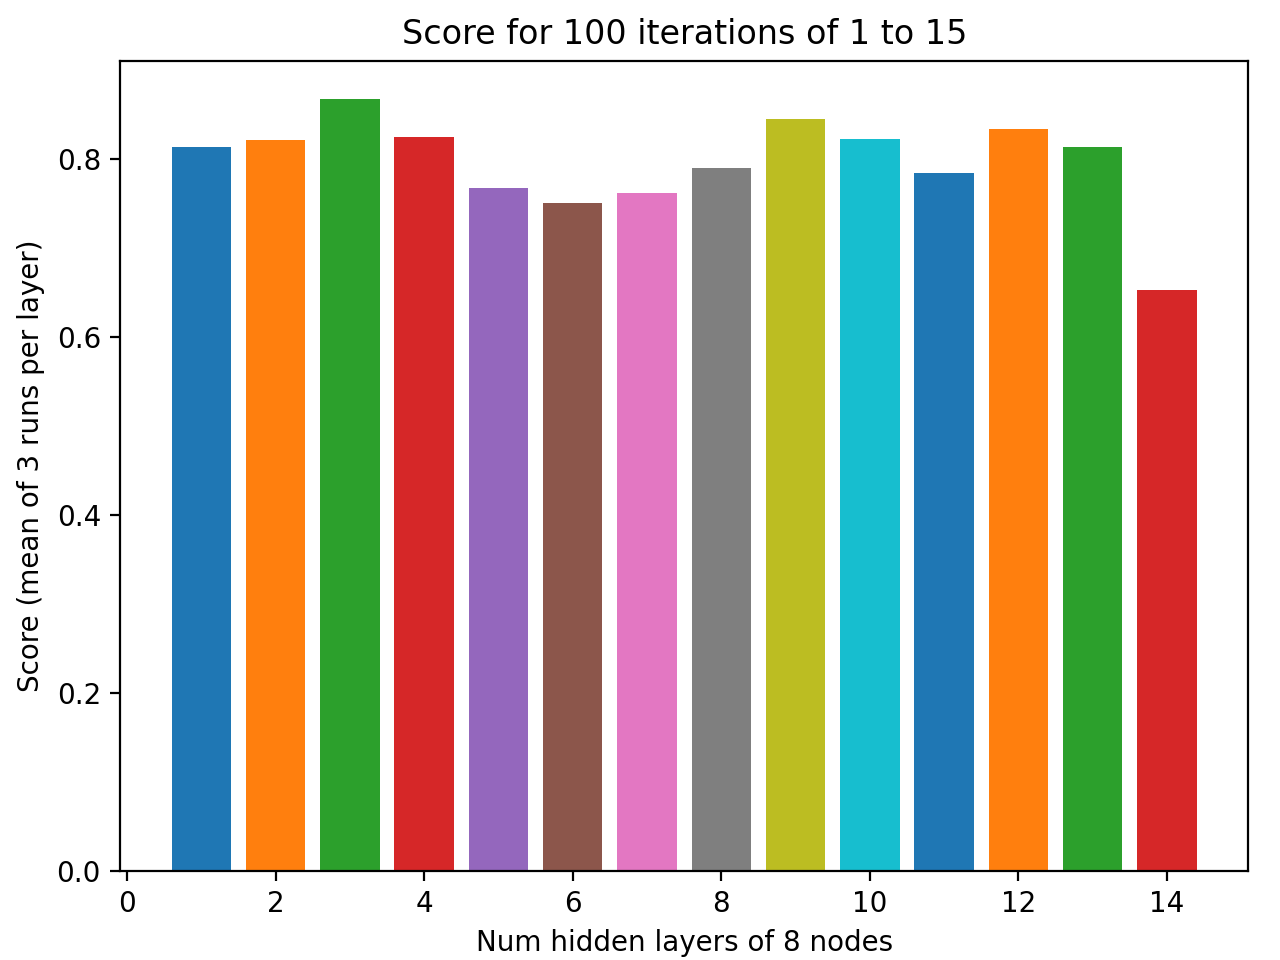
\includegraphics[scale=0.4]{Figure_2-2}

        The graph show that when this model gets more layers (here of just 8 nodes) we see that the score gets worse. I would think this is because the model is trying to learn more then what it should, so it guesses wrong for data that is not in the test data.        

        \paragraph{Accuracy}
        For calculating the accracy I first just calculated the accracy using the \texttt{clf.score(testX, testY)}. This is calculated in the \texttt{runMLPC()}. Afther seeing the data I wrote the \texttt{run()} too allow me to take the mean of \texttt{X} amount of iterations. For this dataset I found it hard to finde some parameters that made the score bad. I think this can be seen in the tables shown. 

        Using the values from the previus tests, 8 nodes in a layer with 6 layres. I show that when the iteratins are low the model is bad, but the model rapidly changes to a "stable" model after it goes true some iterations. Here I am using the \texttt{plotThing1(30, 0, 0, iterationIncreas=10)}. This means that it loops over 30 models and plots their score. Each loop the model iteration is increased by 10 and the first model is iterating 1 time. The score is the mean of 5 runs with the same parameters.

        \begin{center}
            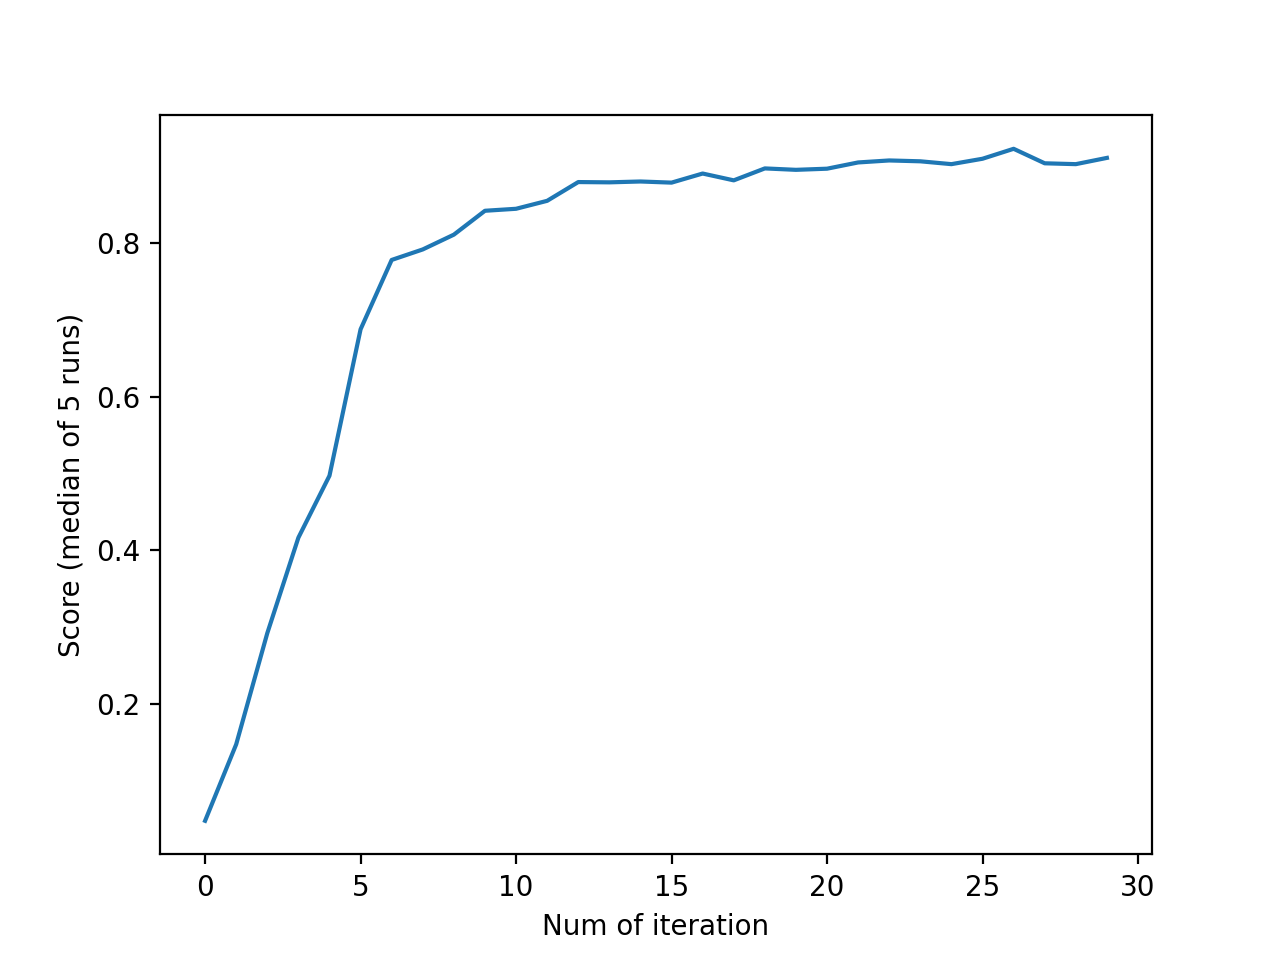
\includegraphics[scale=0.35]{Figure_3}
        \end{center}

        This graf shows that when iterating 150 times seems like a good choice for a good score.

        \paragraph{Conclution}
        It seems like runding this model with 8 nodes in 4 hidden layers and training the model for 150 iterations gives a good score of \texttt{87.78\%}. Increasing any of the parameters will give a better score. I would recomend to change the "number of nodes" and number of iterations.

\end{document}